\section{Methods}
\label{methods_section}

How does a large language model respond when given information that contradicts its inherent knowledge, and why?

To understand this, we need to build a new framework for testing a model's answers when presented with contradictory information.
This framework must be tested with models of various architectures and sizes to get insights about our responses.

Following the example set in \cref{introduction_research_objectives}, we split the work into three sub-objectives.

\subsection{Creating a representative dataset of questions}
\label{creating_dataset}

As argued in \cref{questions_objective}, the research of this thesis requires a large dataset of questions from a variety of categories to test large language models.

\subsubsection{Dataset Description}

The dataset we aim to create for this research is designed to be a comprehensive and versatile tool for evaluating large language models.
By choosing this criteria when selecting questions, we ensure that the dataset will provide meaningful insights of the knowledge grounding of large language models across a wide spectrum of domains.

Our dataset should have the following properties.
\begin{description}[style=nextline]
	\item[1. Questions should have short, unambiguous answers.]
		Our goal is to compare these results for both equality and perplexity. Longer answers make this objective more complicated since two long, correct answers might be equivalent. Shorter answers reduce the space of possible answers that are equivalent, but not equal.
	\item[2. Questions must cover a large and diverse set of topics.]
	    The parametric knowledge of a model comes from a pre-existing dataset of training data, which might be biased towards certain topics or groups of people. For example, it is known that Wikipedia contains a significant geographical bias on biographies \citep{wikipedia_geographic_bias}, and that this affects the probability of giving a correct answer without context \citep{factual_recall}.
		We require a large and diverse and set of topics to counteract potential biases.
	\item[3. Questions must allow for the creation of counterparametric answers.]
		Part of the requirements of this thesis is to allow some tests of contextual versus inherent knowledge.
	    A simple way to do this is to repeat and enhance the approach used by \citeauthor{factual_recall} of adding counterparametric answers to a query context.
		This allows us to to easily disambiguate whether an answer came from the model's memory or from the context.
	    This approach is only possible if the set of answers allows us to create a set of alternative answers that are plausibly correct and have the same format as the parametric answer, but are still counterparametric.
\end{description}

The existing literature uses various existing question-and-answer datasets.
We believe that none of these datasets are a good fit for this research for not following some of the three desired properties.
However, understanding them can be useful when designing the final dataset.

\begin{description}
	\item[Natural Questions Dataset] Created by Google Research \citep{natural_questions}, and commonly used in research related to understanding the answers of LLMs in question-and-answer problems \citep{ragged,when_not_to_trust_llms,can_rag_models_reason}.
		While the dataset provides an excellent range of questions and existing literature to compare these results to, the lack of categorisation is an obstacle in our objective to generate counterparametric answers.
	\item[Human-Augmented Dataset] Sometimes used in research related to quality control of large language models \citep{learning_the_difference}.
		However, the high cost associated with this dataset would limit the size of our questions.
	\item[Countries' Capitals Question Dataset] Used in ``Characterizing Mechanisms for Factual Recall in Language Models'' \citep{factual_recall}, this dataset contains a single question about the capital city of certain countries which can be easily transformed to a counterparametric question.
		This format is ideal for the research done in this thesis, but having a single question pattern will not allow a deep dive into the source of each answer in a general question.
\end{description}

\subsubsection{Dataset Creation}

Instead of using an existing dataset, this research takes inspiration from the paper by \citeauthor{factual_recall} to create a similar but larger dataset of questions and answers from a wide range of topics, where questions can be grouped by question pattern to ensure that their formats are similar.
This way, we can emulate the approach of that paper of using the answer from a certain question as the counterfactual question of another.

This dataset will be used to test the remaining questions of this thesis.
Since it might be useful for future research, it will also be presented as its own result.

To address these items, we follow the approach done by \citeauthor{factual_recall} in creating base questions that refer to a specific object, so all the answers for the same base question have a similar format and creating counterparametric answers is easy.

Since this thesis requires a set of questions that covers a large set of topics, eras, and places, we enhance this method by creating a set of categories, each of which has a large set of base questions and another set of objects that can be matched.
An example of this approach is shown in \cref{source_data_example}.

\begin{table}[htb]
	\setlength{\fboxsep}{0pt}
	\setlength{\fboxrule}{1pt}
	\newcommand{\rep}[1]{{\setlength{\fboxsep}{0pt}\fcolorbox{Gray}{Gray!80}{\textit{#1}}}}

	\centering
	\scriptsize
	\begin{tabular}{>{\bfseries}c | l | c | l}
		\toprule
			\bfseries Category & \bfseries Base Questions & \bfseries Object & \bfseries Queries \\
		\midrule
			Person & \begin{minipage}{.30\textwidth}
				\ttfamily
				Q: What is the date of birth of \rep{\{person\}}? \\ A: The date of birth of \rep{\{person\}} is \\[1ex]
				Q: In what city was \rep{\{person\}} born? \\ A: \rep{\{person\}} was born in
			\end{minipage} &
			\begin{minipage}{.12\textwidth}
				\ttfamily
				\textcolor{Red}{Che~Guevara} \\[1ex]
				\textcolor{Sepia}{Confucius}
			\end{minipage} &
			\begin{minipage}{.40\textwidth}
				\ttfamily
				Q: What is the date of birth of \textcolor{Red}{Che~Guevara}? \\ A: The date of birth of \textcolor{Red}{Che~Guevara} is \\[1ex]
				Q: What is the date of birth of \textcolor{Sepia}{Confucius}? \\ A: The date of birth of \textcolor{Sepia}{Confucius} is \\[1ex]
				Q: In what city was \textcolor{Red}{Che~Guevara} born? \\ A: \textcolor{Red}{Che~Guevara} was born in \\[1ex]
				Q: In what city was \textcolor{Sepia}{Confucius} born? \\ A: \textcolor{Sepia}{Confucius} was born in
			\end{minipage} \\
		\midrule
			City & \begin{minipage}{.30\textwidth}
				\ttfamily
				Q: What country is \rep{\{city\}} in? \\ A: \rep{\{city\}} is in
			\end{minipage} &
			\begin{minipage}{.10\textwidth}
				\ttfamily
				\textcolor{BurntOrange}{Cairo} \\[1ex]
				\textcolor{ForestGreen}{Mumbai} \\[1ex]
				\textcolor{Cyan}{Buenos Aires} \\[1ex]
				\textcolor{Purple}{London}
			\end{minipage} &
			\begin{minipage}{.40\textwidth}
				\ttfamily
				Q: What country is \textcolor{BurntOrange}{Cairo} in? \\ A: \textcolor{BurntOrange}{Cairo} is in \\[1ex]
				Q: What country is \textcolor{ForestGreen}{Mumbai} in? \\ A: \textcolor{ForestGreen}{Mumbai} is in \\[1ex]
				Q: What country is \textcolor{Cyan}{Buenos Aires} in? \\ A: \textcolor{Cyan}{Buenos Aires} is in \\[1ex]
				Q: What country is \textcolor{Purple}{London} in? \\ A: \textcolor{Purple}{London} is in
			\end{minipage} \\
		\bottomrule
	\end{tabular}
	\caption{Some examples of the base-question and object generation that are fed to the models for finding parametric answers.}
	\label{source_data_example}
\end{table}

This list of questions will enable the research on whether the answers given by large language models depend on the category and the format of the questions.

\subsection{Building an experimental framework to understand the source of an LLM's answer}
\label{method22}

\subsubsection{Model Selection}
\label{model_selection}

In order to get a general understanding of large language models with added context, we test the queries generated in \cref{creating_dataset} into four models of different architectures and sizes, which are listed in \cref{model_list}.

\begin{table}[htb]
	\centering
	\begin{tabular}{>{\bfseries}c@{\hspace{20pt}}l l}
		\toprule
			& \bfseries Seq2Seq Model & \bfseries Decoder-Only Model \\
		\midrule
			Smaller & \ttfamily Flan-T5-XL & \ttfamily Meta-Llama-3.1-8B-Instruct \\
			Larger & \ttfamily Flan-T5-XXL & \ttfamily Meta-Llama-3.1-70B-Instruct \\
		\bottomrule
	\end{tabular}
	\caption{The four large language models chosen for this research.}
	\label{model_list}
\end{table}

Both Sequence-to-Sequence models are based on T5 models \citep{t5}, which employ an encoder-decoder architecture: while an encoder processed the input sequence into a context vector, and an decoder generates an input sequence from this vector.
The \texttt{Flan-T5} models are fine-tuned to follow instructions, and have improved zero-shot performance compared to the original T5 models \citep{flant5}.

\texttt{Flan-T5-XL} contains approximately 3 billion parameters, and is considerably bigger than the base Flan-T5 model, which should improve the accuracy of its parametric answers.

\texttt{Flan-T5-XXL} contains 11 billion parameters, so it should have higher accuracy on the parametric answers as the \texttt{XL} model.
However, how the higher amount of parameters will affect the experiments that we are running is still unknown.

Unlike Seq2Seq models, Decoder-only models focus on the generation of text based on the previous tokens.
In a sense, given a sequence of tokens they solve the problem of predicting the following token, repeating sequentially until some final token is found.

These architectures leverages autoregressive attention \citep{attention_is_all_you_need}, where each token attends to its preceding tokens, maintaining the temporal order of the sequence.
This approach allows them to generate coherent and contextually relevant text by sampling from this learned distribution, while also capturing long-range dependencies and complex patterns in language.

The Llama models \citep{llama3} use this architecture and fine-tune it to tasks of instruction-following, and are specially adept at complex prompts.

The Decoder-only model \texttt{Meta-Llama-3.1-8B-Instruct} has 8 billion parameters, while \texttt{Meta-Llama-3.1-70B-Instruct} has 70 billion.
Meta provides an even larger model, \texttt{Meta-Llama-3.1-405B-Instruct}, that is too large to easily experiment with.
However, we expect the difference between this model and the \texttt{70B} model to be roughly the same as the difference between the \texttt{70B} and \texttt{8B} models.

The properties of the models are summarised in \cref{model_card}.

\begin{table}[htbp]
	\centering
	\footnotesize
	\begin{tabular}{>{\ttfamily}l l l r r}
		\toprule
			\rmfamily \bfseries Model & \bfseries Architecture & \bfseries Developer & \bfseries Parameters & \bfseries Context \\
		\midrule
			Flan-T5-XL & Seq2Seq & Google Brain & 3 Billion & 512 Tokens \\
			Flan-T5-XXL & Seq2Seq & Google Brain & 11 Billion & 512 Tokens \\[2pt]
			Meta-Llama-3.1-8B-Instruct & Decoder-Only & Meta AI & 8 Billion & 128k Tokens \\
			Meta-Llama-3.1-70B-Instruct & Decoder-Only & Meta AI & 70 Billion & 128k Tokens \\
		\bottomrule
	\end{tabular}
	\caption{Model cards of the large language models used in this research.}
	\label{model_card}
\end{table}

\subsubsection{What type of answer does each model select for each question?}
\label{methodology_type_of_answer}

The first step to understanding the knowledge grounding of large language models is to create queries that contain counterparametric data as part of the context.
By comparing the result to the existing answers it becomes trivial to understand whether an answer came from the model's memory, the queries' context, or neither of these.

Following the approach of \citeauthor{factual_recall}, for every query we randomly sample from the set of answers of the same base question for answers that are different to the parametric answer which is given by the original query.
An example of this shuffling is in \cref{counterparametric_table}.

Later, we add this \emph{counterparametric answer} to the context, to form a new query and query the same model again; this is exemplified in \cref{category_example}.

To ensure that the results are simple to interpret and minimise the effect of randomness, once we select the queries we follow the example of \citeauthor{ragged} and use Greedy Decoding to find the answer.
While beam search with a short beam width tends to produce more accurate results for long answers \citep{sutskever_seq2seqlearning,wu_mltranslation} and there are many other sampling methods that produce better results \citep{text_degeneration}, this is likely to not have an effect on experiments that result in shorter answers \citep{t5}.

We compare the parametric answer to the previous values to come to one of three cases:
\begin{description}
	\item[\Parametric{}] answers are equal to the answer given by the model when queried without context.
		This answer would come from the parametric memory of the model, and could potentially include hallucinations not fixed by RAG.
	\item[\Contextual{}] answers are equal to the context given in the query.
	\item[\Other] answers are neither of these, and this answer comes from a mis-interpretation of the input by the model or from some other source.
\end{description}

To minimise the amount of problems caused by large language models generating extra information, we define two strings to be equal by removing all text after a period or an \texttt{<EOS>} token, removing punctuation and stop words, and finding whether one is a subsequence of another.

This approach to compare strings is not enough, and understanding whether two answers are identical is an ongoing problem.
This is explained in the Future~Work section in \cref{other_problems}.

The approach to finding out the source of knowledge of each query is specified in \cref{action_diagram}.

\begin{figure}[tb]
	\centering
	\fbox{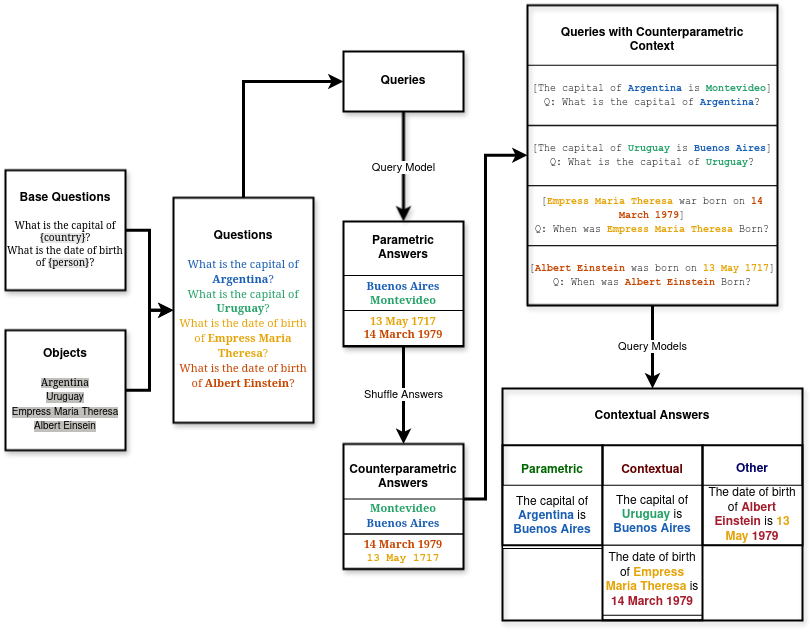
\includegraphics[width=\textwidth]{Method.png}}
	\caption{Example diagram of steps used to calculate the two sets of answers, \textit{parametric} and \textit{contextual}, and to compare them to answer the question in this objective. Many of the terms in this diagram are explained in the \protect\hyperref[glossary]{Glossary}.}
	\label{action_diagram}
\end{figure}

\begin{table}[htbp]
	\centering
	\scriptsize

	\begin{tabularx}{\textwidth}{>{\ttfamily}X >{\ttfamily}c c}
		\toprule
			\bfseries \rmfamily Question with counterparametric context & \bfseries \rmfamily Model Answer & \bfseries Category \\
		\midrule
			\parbox{235pt}{Context: [the nearest major body of water to \textcolor{Mahogany}{Windhoek} is the \textcolor{RoyalPurple}{Rio de la Plata}] \\ Q: What is the nearest major body of water to \textcolor{Mahogany}{Windhoek}? \\ A: The nearest major body of water to \textcolor{Mahogany}{Windhoek} is} &
			\textcolor{Mahogany}{the Atlantic Ocean} &
			\bfseries \textcolor{ForestGreen}{Parametric} \\[22pt]
			%
			\parbox{235pt}{Context: [the date of birth of \textcolor{Red}{Che~Guevara} is \textcolor{Apricot}{965~AD}]. \\ Q: What is the date of birth of \textcolor{Red}{Che~Guevara}? \\ A: The date of birth of \textcolor{Red}{Che~Guevara} is} &
			\textcolor{Apricot}{965~AD} &
			\bfseries \textcolor{Maroon}{Contextual} \\[16pt]
			%
			\parbox{235pt}{Context: [\textcolor{Purple}{Rome} is in \textcolor{Salmon}{Georgia}] \\ Q: What country is \textcolor{Purple}{Rome} in? \\ A: \textcolor{Purple}{Rome} is in} &
			\textcolor{BlueViolet}{the United States} &
			\bfseries \textcolor{MidnightBlue}{Other} \\[12pt]
		\bottomrule
	\end{tabularx}
	\caption{Example for results with \Parametric{}, \Contextual{}, and \Other{} values. Note that, in the third query, the model is interpreting the question as asking about Rome in the US State of Georgia, rather than the country of Georgia.}
	\label{category_example}
\end{table}

\begin{table}[htbp]
	\newcommand{\vwidth}[1]{\parbox{38ex}{\ttfamily #1}}
	\newcommand{\rep}[1]{{\setlength{\fboxsep}{0pt}\fcolorbox{Gray}{Gray!80}{\textit{#1}}}}

	\centering
	\scriptsize

	\begin{tabularx}{\textwidth}{>{\ttfamily}l>{\ttfamily}c@{\hspace{1pt}}>{\ttfamily}c@{\hspace{0pt}}>{\ttfamily}c@{\hspace{10pt}}>{\ttfamily}X}
		\toprule
			\rmfamily \bfseries Base Question & \rmfamily \bfseries Object & \rmfamily \bfseries \parbox{40pt}{\centering Parametric Answer} & \rmfamily \bfseries \parbox{75pt}{\centering Counterparametric Answer} & \rmfamily \bfseries \parbox{120pt}{\centering Question with Counterparametric Context} \\
		\midrule
			\multirow{4}{65pt}[-45pt]{Q: What is the date of birth of \protect\rep{\{person\}}? \\ A: The date of birth of \protect\rep{\{person\}} is} &
			\textcolor{Red}{Che~Guevara} &
			\textcolor{Red}{June~14,~1928} &
			\textcolor{Apricot}{965~AD} &
			\vwidth{Context: [the date of birth of \textcolor{Red}{Che~Guevara} is \textcolor{Apricot}{965~AD}]. \\ Q: What is the date of birth of \textcolor{Red}{Che~Guevara}? \\ A: The date of birth of \textcolor{Red}{Che~Guevara} is} \vspace{2pt} \\
			%
			&
			\textcolor{Apricot}{Ibn~al-Haytham} &
			\textcolor{Apricot}{965~AD} &
			\textcolor{Red}{June~14,~1928} &
			\vwidth{Context: [the date of birth of \textcolor{Apricot}{Ibn~al-Haytham} is \textcolor{Red}{June~14,~1928}]. \\ Q: What is the date of birth of \textcolor{Apricot}{Ibn~al-Haytham}? \\ A: The date of birth of \textcolor{Apricot}{Ibn~al-Haytham} is} \vspace{2pt} \\
			%
			% &
			% \textcolor{Blue}{Boyan~Slat} &
			% \textcolor{Blue}{27~January~1994} &
			% \textcolor{Brown}{February~23,~1868} &
			% \vwidth{Context: [the date of birth of \textcolor{Blue}{Boyan~Slat} is \textcolor{Brown}{February~23,~1868}]. \\ Q: What is the date of birth of \textcolor{Blue}{Boyan~Slat}? \\ A: The date of birth of \textcolor{Blue}{Boyan~Slat} is} \vspace{2pt} \\
			%
			&
			\textcolor{Brown}{W.E.B~Du~Bois} &
			\textcolor{Brown}{February~23,~1868} &
			\textcolor{Red}{June~14,~1928} &
			\vwidth{Context: [the date of birth of \textcolor{Brown}{W.E.B~Du~Bois} is \textcolor{Red}{June~14,~1928}]. \\ Q: What is the date of birth of \textcolor{Brown}{W.E.B~Du~Bois}? \\ A: The date of birth of \textcolor{Brown}{W.E.B~Du~Bois} is} \vspace{2pt} \\
			%
		\midrule
			\multirow{2}{65pt}[-10pt]{Q: What country is \protect\rep{\{city\}} in? \\ A: \protect\rep{\{city\}} is in}
			&
			\textcolor{BurntOrange}{Cairo} &
			\textcolor{BurntOrange}{Egypt} &
			\textcolor{ForestGreen}{India} &
			\vwidth{\vspace{2pt} Context: [\textcolor{BurntOrange}{Cairo} is in \textcolor{ForestGreen}{India}]. \\ Q: What country is \textcolor{BurntOrange}{Cairo} in? \\ A: \textcolor{BurntOrange}{Cairo} is in} \vspace{2pt} \\
			%
			&
			\textcolor{ForestGreen}{Mumbai} &
			\textcolor{ForestGreen}{India} &
			\textcolor{BurntOrange}{Egypt} &
			\vwidth{Context: [\textcolor{ForestGreen}{Mumbai} is in \textcolor{BurntOrange}{Egypt}]. \\ Q: What country is \textcolor{ForestGreen}{Mumbai} in? \\ A: \textcolor{ForestGreen}{Mumbai} is in} \vspace{2pt} \\
		\bottomrule
	\end{tabularx}
	\caption{Using the same question format allows us to repurpose previous parametric answers as counterparametric ones.}
	\label{counterparametric_table}
\end{table}

\clearpage{}

\subsubsection{Understanding the result by finding the mean attention of the context and question areas}

For comparing different architectures, it's useful to understand how much attention they give to the context compared to the rest of the query.

Since all our model architectures employ attention mechanisms \citep{flant5,llama3}, we can estimate the relative importance of tokens in the context and the query by calculating the average self-attention each token receives within its respective section.
Specifically, we compute the mean self-attention weights, which serve as a proxy for the emphasis the model places on different parts of the input.

This approach is formalized in \cref{attention_equation}, where we define the mean self-attention for tokens in the context and query sections.

\begin{equation}
	\newcommand{\lenmod}[1]{\left| \text{#1} \right|}
	\begin{gathered}
		A : \mathbb{R} ^ { \text{batch} \times \lenmod{layer}  \times \lenmod{attn\_head} \times Q \times K } \\[1ex]
		\begin{aligned}
			m_{b,q,k} &= \frac{1}{ \lenmod{layer} \times \lenmod{attn\_head} } \sum^{\substack{\text{layer} \\ \text{attn\_head}}}_{\substack{i = 0 \\ j = 0}} A_{b,i,j,q,k} \\
			d_{b, q} &= m_{b, q, q} \\
			s_{b, i} &= \left(d_{b, i} - \min{\left( d_b \right)}\right) / \left(\max{\left( d_b \right)} - \min{\left( d_b \right)} \right)
		\end{aligned} \\[1ex]
		\text{attn}_\text{ctx} = \frac{1}{\lenmod{ctx}} \sum_{i \in \text{ctx}} s_b_i \qquad
		\text{attn}_\text{rest} = \frac{1}{\lenmod{rest}} \sum_{i \in \text{rest}} s_b_i \qquad
	\end{gathered}
	\label{attention_equation}
\end{equation}

In this equation, $A$ is the 5-tensor representing the attention weights.
$m_{b,q,k}$ represents the mean attention all layers and heads, while $d_b$ represents the diagonal of these attentions which correspond to the self-attentions.

We normalise those values for $s_i$ and average then among the context tokens and the rest of the query, respectively.

\newpage{}

\subsection{Enhancing the framework to understand the reasoning behind each answer}
\label{method_perplexity}

\subsubsection{Perplexity Score}
\newcommand{\NLL}{\text{NLL}}
\newcommand{\PPL}{\text{PPL}}

The Perplexity score of an answer is normally used to measure the inverse of the certainty that the model has of a particular answer \citep{gpt3,retro}.
In a sense, it's the ``surprise'' of a model that a certain answer is correct.

We can define the probability of a model choosing a token $x_n$ with context $x_1, \dots, x_{n - 1}$ from a query $Q$ by calculating the softmax value of all the logits for the possible words for this token.

The probabilities of the tokens if an answer can be accumulated to calculate the negative log-likelihood $\NLL$, which is used to calculate the perplexity $\PPL$ using the formulas from \cref{eq:nll,eq:ppl}.

\begin{align}
	\NLL \left( x_1, \dots, x_n \mid Q \right) &= - \frac{1}{n} \sum^n_{i = 1} \log_2 P \left( x_i \mid Q, x_1, \dots, x_{i - 1} \right) \label{eq:nll} \\[1ex]
	\PPL \left( x_1, \dots, x_n \mid Q \right) &= {2 ^ {\text{NLL} \left( x_1, \dots, x_n \mid Q \right)}} \label{eq:ppl}
\end{align}

% \newpage{}

\subsubsection{Perplexity of the parametric answer with counterparametric context and vice-versa}

Note that the token $x_n$ does not necessarily have to be the result of applying the query $x_1, \dots, x_{n - 1}$ to a model.

Therefore, it becomes necessary to use teacher-forcing \citep{teacher_forcing} to feed some answer to the model regardless of what's the answer to this particular query. This allows us to calculate the perplexity scores of the parametric answers for both the regular query and the one with counterparametric context, and the perplexity scores of the contextual answers for these two queries.

For a given parametric answer $p_1, \dots, p_n$ and randomly sampled counterparametric answer $q_1, \dots, q_m$, a query without context $Q$, and a query with this counterparametric context $Q'$ we can calculate four different perplexity scores as shown in \cref{perplexity_table}.

\begin{table}[hbt]
	\footnotesize
	\centering

	\renewcommand{\arraystretch}{3}
	\begin{tabular}{  l >{\centering}p{.2\textwidth} | >{\centering}p{.3\textwidth} | p{.3\textwidth} | }
		\cline{3-4}
			& & \multicolumn{2}{c|}{\raisebox{11pt}{\bfseries Tokens}} \\[-15pt]
		\cline{3-4}
			& & \raisebox{11pt}{Parametric $p$} & \raisebox{11pt}{\hspace{20pt} Counterparametric $q$} \\[-15pt]
		\hline
			\multicolumn{1}{ | c | }{\multirow[b]{2}{*}{\rotatebox{90}{\bfseries \centering  Context}}}
			& Base Query &
			$P_0 = \PPL \left( p_1, \dots, p_n \mid Q \right)$ &
			$P_1 = \PPL \left( q_1, \dots, q_{m} \mid Q \right)$ \\
		\cline{2-4}
			\multicolumn{1}{ | c | }{} & Counterparametric Context &
			$P_2 = \PPL \left( p_1, \dots, p_n \mid Q' \right)$ &
			$P_3 = \PPL \left( q_1, \dots, q_{m} \mid Q' \right)$ \\
		\hline
	\end{tabular}
	\caption{Four different perplexity values: one for each set of tokens, and one for each query context.}
	\label{perplexity_table}
\end{table}

Since the parametric answer is by definition the response of the model to the regular query, $P_0 \leq P_1$.
In fact, the perplexity of the parametric value is lower than the perplexity of any other answer on query $Q$.

\Cref{example_perplexity} contains an example of the calculation of the perplexity values for a particular query.

\subsubsection{Predicting whether an answer came from memory or from context}

One question remains: if the response of the query with counterparametric context $Q'$ is a certain answer $x_1, \dots, x_n$, how can we predict whether this answer is came from the model's memory $p$ or from the given context $q$ without requiring an extra query?

We propose investigating the value of the perplexity $\PPL \left( x_1, \dots, x_n \mid Q' \right)$ and comparing it to the distribution of perplexities on the answers with added parametric context $P_2$ and $P_3$.
For simplicity reasons, we are obviating the case when the preferred answer is neither of these; instead, we focus on whether the parametric or counterparametric answer are more likely.\footnotemark{}

\footnotetext{TODO: Maybe include a KDE or a K-S test here.}

\begin{figure}[p]
	\centering
	\scriptsize

	\newcommand{\tokbox}[1]{\fbox{\strut\centering #1}}

	\begin{minipage}{.47\textwidth}
		\centering \textbf{Base Query} $Q$ \\ \fbox{\parbox[][6em]{\textwidth}{\ttfamily Q: Where is The Son of Man primarily housed? \\ A: The Son of Man is currently in}}
	\end{minipage} \hfill{}
	\begin{minipage}{.47\textwidth}
		\centering \textbf{Query with Counterparametric Context} $Q'$ \\ \fbox{\parbox[][6em]{\textwidth}{\ttfamily [Context: The Son of Man is housed in in the refectory of the Convent of Santa Maria delle Grazie in Milan, Italy] \\ Q: Where is The Son of Man primarily housed? \\ A: The Son of Man is currently in}}
	\end{minipage} \\[1em]

	\begin{minipage}{.47\textwidth}
		\centering \textbf{Parametric Answer Tokens} $p_1, \dots, p_n$ \\ \fbox{
			\parbox[][6em]{.98\textwidth}{
				\ttfamily
				\tokbox{ the}\tokbox{ collection}\tokbox{ of}\tokbox{ the}\tokbox{ National}
				\tokbox{ Gallery}\tokbox{ of}\tokbox{ Canada}\tokbox{ in}\tokbox{ Ottawa}\tokbox{,}
				\tokbox{ Ontario}\tokbox{,}\tokbox{ Canada}
			}
		}
	\end{minipage} \hfill{}
	\begin{minipage}{.47\textwidth}
		\centering \textbf{Counterparametric Answer Tokens} $q_1, \dots, q_m$ \\ \fbox{
			\parbox[][6em]{.98\textwidth}{
				\ttfamily
				\tokbox{ the}\tokbox{ ref}\tokbox{ect}\tokbox{ory}\tokbox{ of}\tokbox{ the}\tokbox{ Con}\tokbox{vent}
				\tokbox{ of}\tokbox{ Santa}\tokbox{ Maria}\tokbox{ delle}\tokbox{ Graz}\tokbox{ie}
				\tokbox{ in}\tokbox{ Milan}\tokbox{,}\tokbox{ Italy}
			}
		}
	\end{minipage} \\[1em]

	\begin{minipage}{.47\textwidth}
		\centering $P \left( p_i \mid Q', p_1, \dots, p_{i - 1} \right)$  \\ \fbox{
			\parbox[][6em]{.98\textwidth}{
				\ttfamily
				\tokbox{0.94}\tokbox{4e-05}\tokbox{0.87}\tokbox{0.93}\tokbox{0.06}
				\tokbox{0.92}\tokbox{0.26}\tokbox{0.04}\tokbox{0.61}\tokbox{0.98}\tokbox{0.72}
				\tokbox{0.49}\tokbox{0.59}\tokbox{0.90}
			}
		}
	\end{minipage} \hfill{}
	\begin{minipage}{.47\textwidth}
		\centering $P \left( q_i \mid Q', q_1, \dots, q_{i - 1} \right)$ \\ \fbox{
			\parbox[][6em]{.98\textwidth}{
				\ttfamily
				\tokbox{0.94}\tokbox{0.96}\tokbox{0.99}\tokbox{1.00}\tokbox{0.98}\tokbox{0.99}\tokbox{0.99}\tokbox{1.00}
				\tokbox{0.99}\tokbox{0.99}\tokbox{0.99}\tokbox{0.99}\tokbox{0.99}\tokbox{0.99}
				\tokbox{0.96}\tokbox{0.99}\tokbox{0.98}\tokbox{0.99}
			}
		}
	\end{minipage} \\[1em]

	\begin{minipage}{.47\textwidth}
		\centering $\NLL \left( p_1, \dots, p_n \mid Q' \right)$  \\ \fbox{
			\parbox[][6em][]{.98\textwidth}{
				\begin{equation*}
					- \frac{1}{n} \sum^n_{i = 1} \log_2 P \left( p_i \mid Q', p_1, \dots, p_{i - 1} \right) = 2.0566
				\end{equation*}
			}
		}
	\end{minipage} \hfill{}
	\begin{minipage}{.47\textwidth}
		\centering $\NLL \left( q_1, \dots, q_m \mid Q' \right)$  \\ \fbox{
			\parbox[][6em][]{.98\textwidth}{
				\begin{equation*}
					- \frac{1}{n} \sum^m_{i = 1} \log_2 P \left( q_i \mid Q', q_1, \dots, q_{i - 1} \right) = 0.0154
				\end{equation*}
			}
		}
	\end{minipage} \\[1em]

	\begin{minipage}{.47\textwidth}
		\centering $P_2 = \PPL \left( p_1, \dots, p_n \mid Q' \right)$  \\ \fbox{
			\parbox[][6em][]{.98\textwidth}{
				\begin{equation*}
					P_2 = 2 ^ {\displaystyle \NLL \left( q_1, \dots, q_m \mid Q' \right)} = 4.1599
				\end{equation*}
			}
		}
	\end{minipage} \hfill{}
	\begin{minipage}{.47\textwidth}
		\centering $P_3 = \PPL \left( q_1, \dots, q_m \mid Q' \right)$  \\ \fbox{
			\parbox[][6em][]{.98\textwidth}{
				\begin{equation*}
					P_3 = 2 ^ {\displaystyle \NLL \left( q_1, \dots, q_m \mid Q' \right)} = 1.0107
				\end{equation*}
			}
		}
	\end{minipage} \\[1em]

	\fbox{\parbox[][6em]{\textwidth}{
		\begin{equation*}
			P_2 > P_3 \qquad \Longrightarrow \qquad \text{\Contextual{}}
		\end{equation*}
	}}

	\caption{Example of perplexity calculation for the parametric and counterparametric answers in a query with the counterparametric context. Note that, due to teacher forcing, the calculation finds the probability of the next token $p_i$ \textit{given the previous tokens of the searched answer $p_1, \dots, p_{i - 1}$} rather than given the most likely tokens. For example, once we feed the string ``\texttt{National Gallery of Canada in}'', the probability of the next token being ``\texttt{Ottawa}'' is very high. In the same way, despite the perplexity of the word \texttt{collection} following \texttt{the} is very high, the perplexity of the following words is considerably lower.}
	\label{example_perplexity}
\end{figure}

